%\documentclass[12pt]{book}
\documentclass[12pt]{article}
% This work is about rootkits
%\usepackage[T2A]{fontenc}
\usepackage[utf8]{inputenc}
\usepackage{multicol}
\usepackage{gensymb}
\usepackage{graphicx}
\usepackage{listings}
\usepackage{verbatim}

\usepackage{hyperref}
\hypersetup{colorlinks, 
           citecolor=black,
           filecolor=black,
           linkcolor=black,
           urlcolor=black,
           bookmarksopen=true,
           pdftex}

\hfuzz = .6pt % avoid black boxes

% TODO List
%\usepackage{color}
%\usepackage{index} % use index package to create indices
%\newindex{todo}{tod}{tnd}{TODO List} % start todo list
%\newindex{fixme}{fix}{fnd}{FIXME List} % start fixme list
%\newcommand{\todo}[1]{\textcolor{blue}{TODO: #1}\index[todo]{#1}}
%\newcommand{\fixme}[1]{\textcolor{red}{FIXME: #1}\index[fixme]{#1}}

\title{Kernel rootkits in Linux: low-level approach and prevention}
\date{}
\author{Ivan Galinskiy}

\begin{document}
\maketitle
  \emph{
  Copyright (C) 2010 Ivan Galinskiy.
    Permission is granted to copy, distribute and/or modify this document
    under the terms of the GNU Free Documentation License, Version 1.3
    or any later version published by the Free Software Foundation;
    with no Invariant Sections, no Front-Cover Texts, and no Back-Cover Texts.
    A copy of the license is included in the section entitled "GNU
    Free Documentation License".}

  \section{A little disclaimer}

  This work is mostly the representation of the process of learning
  system internals.
  
  \section{Kinds of rootkits}
  \subsection{Classification}
  What exactly are the rootkits? In the malware classification, rootkits are
  programs designed to hide the fact of system intrusion by hiding processes,
  users, files etc. This is the base classification, which is true for all
  kinds of rootkits. But if we look at real samples, deviations appear. For
  example, in some cases the rootkit is not just ``standalone'', but a part of
  another piece of malware which is being hidden. A very good example is
  Rustock.C designed for Windows.

  \subsection{Basic principles of work}
  Obviously, the process of hiding something is based on modifying system
  ``internals'', requiring thus some way to gain administrative (root)
  privileges. This can be done in very different ways, and besides, it is not
  part of rootkit's job, so we will skip that. But there are basically two
  ways the rootkit ``holds'' itself on the main system:
  \begin{enumerate}
    \item Modifying files on the filesystem. When a program has administrative
      rights on the target machine, it can (almost always) do whatever it
      ``wants''. For example, modifying the passwd or sudo utilities will
      probably get users' passwords. The disadvantages are obvious. To detect
      the rootkit, the user needs to check main utilities' checksums from a
      trusted operating system (either by loading with LiveCD or by taking the
      harddisk to another machine).

    \item Modifying only the RAM. Of course, at first sight it may look a bit
      strange, as with a reboot anything will return to normal. But just
      imagine a server with, lets say, 2 years uptime? Now it looks better,
      and this kind of rootkits is much tougher (and more interesting to
      research).
  \end{enumerate}

  \section{A brief look at DR Linux rootkit}
  
  Well, finding this one was not a difficult task. Besides, it's one of the
  most up-to-date open-source rootkits available. Others are either very old,
  or don't match our context, so we will not look at them. The source code
  indicates that this rootkit is based on debug registers. According to Intel
  documentation, the debugging registers are DR0 - DR7. DR0 - DR3 registers
  hold four linear addresses. DR4 and DR5 are reserved for extended debugging
  and we are not going to look at them now. DR6 is the ``Debug State
  Register'' and DR7 is the ``Debug Control Register''. What is their purpose?
  The below scheme from Intel documentation explains some things.
  \begin{figure}[h]
    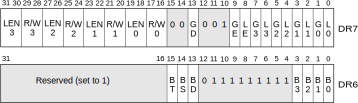
\includegraphics[width=\linewidth, keepaspectratio]{dregs}
  \end{figure}
  The one interesting is the DR7, which controls the debugging behaviour. For
  the rootkit, the usefullness is in the ability to control read, write or
  execute operations (or their combinations) on the breakpoints (note: the
  settings are individual for each breakpoint). Obviously, the breakpoints are
  not useful by themselves. When a breakpoint is reached, after executing it,
  the processor emits a \verb!#DB! exception, which is catched by the kernel
  handler in normal cases. But the rootkit changes the handler in Interrupt
  Descriptor Table to its own or either modifies the system handler (in this
  case the IDT remains untouched).

  \section{Interception techniques}

  Wait, is this the only way to control system internals? Actually, more
  methods were created through the time, but all of them are based on
  modifying well-known system structures, the quantity of which is not so
  big. What structures? Some of them are IDT, MSR, DR registers (as seen
  above), syscall tables... What are all these abbreviatures? They may look
  scary at first sight, but the things are simpler. So what all those things
  do?

  \begin{itemize}
    \item IDT means Interrupt Descriptor Table. In simple words, it contains
      addresses of handlers for interrupts. As we have seen in the DR rootkit,
      it may be very useful. There is also another detail, before Pentium II
      was introduced, system calls (i.e. calls from user applications to
      kernel) were performed using the \verb!0x80!  interrupt (loading the
      system call number into EAX register before invoking interrupt). And
      guess what? The pointer to the handler for that interrupt was stored in
      IDT too.

    \item MSR stands for Model Specific Registers. Before Pentium II,
      interrupts were used to make system calls. It's a simple way, but
      unfortunately, slow. That's why \verb!SYSENTER/SYSCALL! and
      \verb!SYSEXIT/SYSRET! (for Intel/AMD respectively) commands were
      introduced, providing a faster way to make system calls. Now the pointer
      to that handler of the call was not in IDT, but in a set of MSR
      registers. They store the target instruction, stack segment pointer
      etc. But the most interesting and useful for us is the
      \verb!IA_32_SYSENTER_EIP! which stores the target instruction. Changing
      it to something else will redirect all the system calls into the new
      procedure.

    \item So what is the difference between the above two methods? Only the
      way to \emph{call} system procedures! Even if we examine the source of
      \verb!system_call! and \verb!ia32_sysenter_target! (there is where
      \verb!IA_32_SYSENTER_EIP!  points by default), in both we find
      ``\verb!call *sys_call_table(,%eax,4)!''. This means that those
      procedures are the same in both cases (otherwise, it would be
      strange). And, of course, modifying pointers in this table can be very
      funny for the rootkit (and more for the machine owner).
  \end{itemize}


  \subsection{Modifying IDT}
  There are some other ways, of course, but now we will concentrate on the
  ones listed above and try to perform these ``tricks''. So, the first in the
  list is interception of interrupts via IDT. Ok, let's begin.
  \begin{itemize}
    \item First of all, I am going to be as kernel version independent as I
      can. It means that I am going to use resources available in the
      processor rather that predefined macros or whatever.
      
    \item OK, before we make any changes to IDT, we obviously need to know
      where exactly it resides. An assembly command \verb!SIDT! can help us
      with this, getting the IDTR register contents. In 32-bit systems, IDTR
      contains two fields: the 16-bit limit, specifying the size of the table,
      and 32-bit address which is the location of IDT. But there is a detail
      that led me to mistakes: the address is stored with low-order bytes
      first! We can define a function to get the register contents in
      easily-readable form: \verbatiminput{sidt.h}

    \item Half of the job is done now. However, we still need to get a
      particular entry in the IDT (to store the original interrupt handler,
      for example). In Linux on 32-bit systems, each entry in IDT is 8-bytes
      long and consists of an offset to the handler and some attributes. The
      funny thing is the offset is not continuous in the entry! The first 16
      bits begin at bit 0 of the IDT entry, and the last 16 are at the end of
      the entry. Tricky, right? The following code can handle with this:
      \verbatiminput{idt.h}

    \item Very good! Now that we have the entries, many things can be
      done. But let's stop with IDT hooking and continue to the next method.
  \end{itemize}

  \subsection{SYSENTER/SYSCALL interception}
  Well, this one is a juicy one! As I already told, beginning with Pentium II,
  Intel processors implemented the new \verb!SYSENTER!/\verb!SYSEXIT!
  instructions (and AMD used \verb!SYSCALL!/\verb!SYSRET!). They decreased the
  overhead of switching from user mode and vice-versa (the interrupts are
  slow). These instructions used special MSR registers to know where the
  target procedure was located. There is one that is specially relevant to us:
  \verb!SYSENTER_EIP_MSR!. Its contents are loaded to the EIP register
  (basically a jump) at the end of \verb!SYSENTER! execution. Initially it
  points to a kernel procedure, but we can change it to our procedure. How can
  it be done?
  \begin{itemize}
    \item First, of course, we need a way to access the
      \verb!SYSENTER_EIP_MSR! register. It's not accessed like the, let's say,
      EAX register. There is a special instruction, \verb!RDMSR!, that does
      it. The only requirement is that the number of MSR register should be
      loaded into ECX (the number of \verb!SYSENTER_EIP_MSR! is 0x176). The
      contents are stored in EDX and EAX registers (EDX is 0 on 32-bit
      systems).
      
    \item Now we can put a new value to the register. This process is
      basically an inverted version of the previous. We load the new value
      into EDX:EAX (EDX is zero, EAX is the new procedure pointer), the MSR
      register number into ECX, and perform the instruction \verb!WRMSR!.
  
    \item I thought that an example would be more helpful than a dry
      description, so here is a minimal sample kernel module for this task
      (the includes were (duh) excluded). It's a kernel module because
      \verb!WRMSR!  can only be performed at ring 0: \verbatiminput{msr.h}
      
    \item Obviously, this module doesn't do anything special, it's more like a
      ``proof-of-concept''. But the payload will come later.
  \end{itemize}

  \section{Designing a rootkit}
  
  Now we have the most popular methods of intercepting system internals, which
  are also pretty easy to detect. Usually the check consists of retrieving the
  system structures, registers etc. and comparing them to the original ones
  found in an uncompressed kernel (or the System.map file). Can the results of
  such a check be trusted? No! The rootkits now prefer to modify the system
  handlers themselves instead, as it's more difficult to discover. For
  example, let's see the method for debugging registers (it's simpler than
  other methods), but in a new way.

  \subsection{Modifying the original debug handler}
  \begin{enumerate}
    \item What happens when a breakpoint is reached? The 0x1 interrupt. Now we
      need to see what procedure is called to handle that interrupt, so let's
      see the IDT.

    \item On my system, it reported the address 0xc125af80. This doesn't tell
      a lot, right? To discover what it is, I used the System.map file. The
      result was a function ``\verb!debug!''. Now this is interesting! Let's
      see what this function does in kernel sources. Actually, the debug entry
      is located (kernel 2.6.33) in the \verb!arch/x86/kernel/entry_32.S! (was
      tricky to find). And this is the code.  \verbatiminput{deb_entry.S}

   Good! The ``\verb!call do_debug!'' seems to be the call to the
   ``official'' debug handler. And if we change it with our own handler,
   which then gives control to \verb!do_debug!? Lots of fun! The only
   problem here is that we actually need to find this call and replace the
   original address to our own handler.

   \item Yes, in theory it's simple, but the practice is a bit more
     complicated. It should be good to see part of disassembled listing of
     ``\verb!debug!'':
     \verbatiminput{debug.s} Interesting, right? But here is a problem. As the
     hex code of ``\verb!call!'' in this case is \verb!0xe8!, it's a relative
     near call. Obviously, it's not acceptable for the hooking function (the
     addresses will be different), so first we need to calculate the absolute
     offset of ``\verb!do_debug!''. Yes, and just for clarity: the 4-byte
     value after ``\verb!0xe8! is a signed integer. The offset is added to the
     address of the next instruction, in my case \verb!0xc125afd0!, and
     (voilà!) we obtain the linear address of ``\verb!do_debug!''. But first,
     we need to find this call. According to the objdump listing provided
     above, the 4-byte pattern we are looking for is
     \verb!0xd289e0e8!. Digging in the kernel is hard for a human, so let's
     define another function.  \emph{Important: when we get a value from
       memory and use it as an integer, it's inverted (because of the
       endianness). So if we need to find code, we need to invert the pattern
       again}: \verbatiminput{search.h} \emph{WARNING: It's not the best or
       the fastest code, but considering that it will usually be called only
       once, it's not critical}
  \end{enumerate}
  Well, this is a good technique, but I will not use it because of the
  relatively easy way to access DR0-DR7 registers. Instead, I will use a
  little bit more complicated, but more reliable (in terms of ease of
  discovery) method of hijacking system calls directly in the
  \verb!sys_call_table!.

  \begin{itemize}
  \item The responsible code, found both in \verb!system_call! and
    \verb!ia32_sysenter_target! (what additionally proves that system calls
    are located in that table), is \verb!call *sys_call_table(,%eax,4)!. This
    is the disassembled fragment of \verb!ia32_sysenter_target!:
    \verbatiminput{syscall_dis.S} A negative value?  It cannot be, since the
    opcode \verb!0xff! always means an absolute offset. It's a mistake in
    \verb!objdump!, so I sent a bug report. However, it's not that critical,
    and we may continue.

  \item Now the function ``\verb!search!'', defined above, can be used to
    search the pattern \verb!0x00ff1485! (taken from the disassembly listing),
    and that is how we obtain the address of \verb!sys_call_table!!

  \item Well, the table is here, but we have no idea on what entry is
    interesting for us. But there is a very useful file in kernel sources,
    \verb!arch/x86/kernel/syscall_table_32.S!. I will provide a little
    fragment of that file: \verbatiminput{syscall_table.S}

  \item Why waiting?! Let's have some fun and modify the \verb!sys_open!!
    First, I would like to define a function to find \verb!sys_call_table! and
    a inline function to read a particular entry. Here they go:
    \verbatiminput{syscall.h}

  \item Now that we have all the nessesary addresses, \verb!sys_open! can be
    ``patched''. How? I found it easier to read the disassembled listing of
    \verb!sys_open! (again, right?) than searching through the kernel
    source. Also the function is not so big, so you may see the complete
    listing of it: \verbatiminput{sys_open.S} Why so tiny? Looks more like a
    wrapper or something similar. And it is! Look at the
    ``\verb!call 0xc10b0307!'' (\verb!0xe8! opcode, another relative
    offset). In my system this address represents function
    ``\verb!do_sys_open!''. Feeling the power? Oh yes.

  \item So, now it's only a question of technique to hook
    \verb!sys_open!. After that the function \verb!search!, a pointer to the
    beggining of the address (or better said, relative offset) is
    obtained. This offset is stored as a signed integer, after that we obtain
    the address of the next instruction by adding 4 (4 bytes) to the
    pointer. Then the offset is added to that pointer and that is how we
    obtain the absolute offset of ``\verb!do_sys_open!''. Well, it's not that
    simple. Why? The pages that contain this code are write-protected, so an
    attempt to write there will cause an exception and nothing more (it took
    me some time to figure it out). But there is the WP bit in CR0 register
    which enables/disables write protection, so we can use it in the following
    helper function:\verbatiminput{rw_protect.h}
    Problem solved! The complete module code will look like this:
    \verbatiminput{open_hook.c}

  \item Let's now modify the hook in such a way that it will block
    access to, for example, all the filenames ending with ``st''. It's
    not pretty useful, but it shows some principles. But as we are
    replacing the \verb!do_sys_open! call, we will take the
    \verb!do_sys_open! definition in kernel sources as a base for our
    hook. So the modified hook looks like
    this:\verbatiminput{open_hook_inter.c} Don't pay attention to the
    strange way of checking filename ending. The reason for this is
    that the name is provided to \verb!open! in different ways, and
    that function then calls \verb!getname! to determine full
    filename, but I am not going to work with it right now, because I
    was only showing the technique itself.
  \end{itemize}

\section{Detection}
Now that the basic principles are known, we can finally develop an
application that will detect hijacking attempts \emph{before} any
damage can be done to the OS and possibly discover existing
rootkits. The functions of that ``IDS'' will be the following:
\begin{enumerate}
  \item At startup, read the \verb!GDTR!, \verb!IDTR!, \verb!SYSENTER_EIP_MSR!
    registers.
    
  \item Retrieve the values of debugging registers and, if
    a ``suspicious'' value is found, do something.
    
  \item A good technique of hiding something is by clearing the P flag
    of that ``something''. I mean, the page will look like it's not
    present in the memory and the \#PF exception will be raised, which
    is then caught by the handler. The handler itself can be
    malicious, permitting it to intercept things.

  \item Retrieve \verb!ia32_sysenter_target! and \verb!system_call! in
    order to compare them to the version found in vmlinux.

  \item Retrieve GDT. The rootkit may add descriptors with base not
    equal to zero and use them in order to make the disassembly much
    more complicated, but becoming more detectable.

  \item Retrieve \verb!sys_call_table!, all the system calls, the IDT
    and the interrupt handlers (especially the \#PF handler).

  \item Clear the P flag on some ``attractive'' system structures. Why
    the P flag instead of debugging registers? Well, the debugging
    registers can be modified very easily, that's the reason. It's
    more complicated, of course, but gives more reliability. Here I am
    going to use a predefined kernel function to ensure compatibility
    and portability.
\end{enumerate}
Well, it's not such a large list, so let's begin.I think it might be
better to first make the IDT handlers' comparison function. But there
is a little thing about finding the end of the interrupt handler,
because we are going to need something like a disassembler. This time
I am going to use a ready disassembler engine called ``hde32'',
written by Vyacheslav Patkov. I found it simple enough for my task,
that is the reason of my choice (others disasm engines were a little
big). Here is how the usage will look like: \verbatiminput{idt_compare.h}
Let's leave it for later and try to solve other requirements.

%\printindex[todo]
%\newpage
%\appendix
%\section{GNU Free Documentation License}
%\input{license.tex}
\end{document}
